\chapter{Strategie testowania oprogramowania}
Projekt informatyczny określa zasady tworzenia i wykonywania testów. Zasady te mają na celu dostarczenie produktu, którego jakość spełnia założone wymagania. Wymagania te są zróżnicowane w zależności od charekterystyki produktu to jest, systemy medyczne, bankowe, telekomunikacyjne wymagają krytycznie wysokiej jakości, aplikacje internetowe natomiast cechują się mniej restrykcyjnymi normami. Zbiór reguł i praktyk nazywamy strategią. Strategia testowania oprogramowania determinowana jest głównie przez dwa aspekty: wspomniana wcześniej charakterystyka produktu i model tworzenia oprogramowania. 
Jak już zostało wspomniane strategia określa sposób tworzenia i wykonywania testów, określa również harmonogram i tryb pracy zespołu testerskiego.

\label{cha:strategie testowania}
\section{Testowanie w procesie tworzenia oprogramowania}
\label{sec:testowanieWprocesie}
Model tworzenia oprogramowania jest to usystematyzowany proces opisujący jakie kroki (zwane fazami) muszą zostać podjęte w celu stworzenia nowego produktu, bądź nowej wersji produktu. Model determinuje między innymi kolejność faz, ich częstotliwość, czas trwania, możliwość powrotu do faz wcześniejszych. Jedną z faz projektu informatycznego jest faza testowania. W zależności od modelu tworzenia oprogramowania, faza testownia przyjmuje postać całkowicie oddzielnej lub zintegrowanej z innymi wcześniejszymi fazami. Model określa również specyfikę testów które powinny być wykonane  i czas kiedy prowadzone jest projektowanie i analiza testów.
Można wydzielić dwa typy modeli tworzenia oprogramowania: klasyczne i zwinne.  
\section{Modele tradycyjne}
Modele tradycyjne zakładają dokłade zdefiniowanie projektu i wykonanie go według liniowo ustalonej kolejności.
\subsection{Model Kaskadowy}
Model kaskadowy powstał w celu ujednolicenia faz potrzebnych do stworzenia oprogramowania. Zakłada iż każda faza następuje po zakończeniu poprzedniej, przy czym przed przejściem do kolejnej fazy nastąpić musi weryfikacja poprzez spełnienie kryterium wyjścia \cite{SEaT}. Model ten zakłada pełną specyfikacja wymagań i zaprojektowanie systemu przed implementacją. Pełna definicja wymagań ułatwia zaprojektowanie fazy testowej gdyż dane wejściowe są znane. W modelu tym nie występują błędy związane ze zmianą wymagań podczas implementacji. Z drugiej strony restrykcyjne przestrzeganie pierwotnych założeń powoduje iż projekt pomimo pozytywnej weryfikacji nie przechodzi fazy walidacji. Naturą projektów informatycznych jest zmiana, natomiast model kaskadowy nie jest otwarty na zmiane wymagań. 
\begin{figure}[h]
\centerline{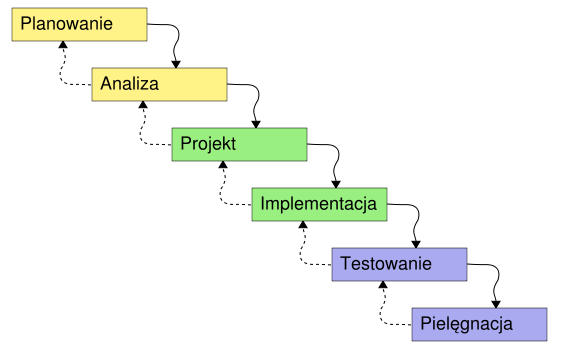
\includegraphics[scale=0.5]{img/model_kaskadowy.png}}
\caption{Model kaskadowy}
\label{fig:kaskadowy}
\end{figure}

Istnieją różne podejścia do testowania w modelu kaskadowym. Pierwsze teoretyczne poddejście zakłada ścisłe rozdzielenie fazy implementacji od fazy testów co oznacza iż nie wykonywane są nawet testy modułowe. Drugie podejście zakłada podczas fazy implementacji wykonywanie testów modułowych i statycznej weryfikacji.

Model kaskadowy stosowany jest głównie dla dobrze zdefiniowanych projektów, najczęściej w segmentach bezpieczeństwa publicznego ponieważ przejście pomiędzy fazami może być połączone z przeglądem i akceptacją formalnych dokumentów

Rozdzielenie faz implementacji od fazy testowania powoduje nierównomierną alokację pracowników. Podczas fazy implementacji pracuje zespół programistyczny który tworzy cała pulę kodu. Zespół ten praktycznie nie jest potrzebny podczas fazy testowania podczas której pracę rozpoczyna zespół zapewnienia jakości.
\begin{figure}[h]
\centerline{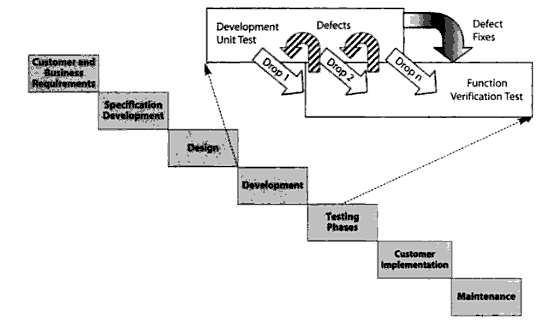
\includegraphics[scale=0.5]{img/water-wheel.png}}
\caption{Model kaskadowy, podział na części}
\label{fig:kaskadowyCzesci}
\end{figure}

Jedną z wariacji modelu kaskadowego jest rozbicie tworzonego oprogramowania na części \cite{TestingMatt}. 
Zespół programistyczny oddaje pierwszą część do testów. Wykonywane są testy integracyjne i testy systemowe natomiast znalezione błędy konsultowane są z zespołem programistycznym i zgłaszane. Równolegle zespół programistyczny pracuje nad poprawą zgłoszonych błędów i dokończeniem implementacji części systemu które nie zostały oddane w pierwszej cześci. Kolejna oddana część jest poddawana testom, weryfikacji poprawionych błędów i małej regresji.

 
 
\subsection{Model V}

\begin{figure}[h]
\centerline{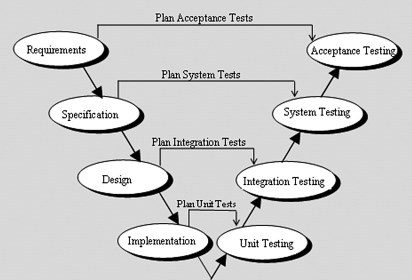
\includegraphics[scale=0.5]{img/vmodel.png}}
\caption{Model V}
\label{fig:vmodel}
\end{figure}
Model V zakłada rozpoczęcie czynności związanych z planowaniem fazy testów równolegle z fazami analizy, projektu i implementacji. Model obrazuje litera V dla której lewa część to czynności związane z implementacją i planowaniem a prawa część to czynności powiązane z testami. Model zakłada iż każdy typ testu jest połączony z jedną fazą z lewej części modelu. Oznacza to iż fazy zbierania wymagań, analizy, projektu i implementacji oprócz swoich specyficznych artefaktów dostarczają także analizę wymagań, scenariusze, przegląd dokumentów i kryteria sukcesu do odpowiednich faz testów.
Pozytywnym aspektem modelu V jest to iż podczas początkowych faz zaangażowany jest zespół testerski który aktywnie uczestniczy w opisanych wsześniej czynnościach. Wadą modelu jest to iż rola zespołu testerskiego ograniczona jest do biernego przyjmowania artefaktów bez możliwości ich wstępnej walidacji.  Według Rex Black, model ten sterowany jest głównie poprzez koszty i harmonogram.
\paragraph{}
Model ten zakłada iż kolejność nie jest stała jak w modelu kaskadowym. każda  faz może spowodować powrót do fazy wcześniejszej, tak więc wymagania mogą ulec zmianie. Zmiana wymgań powoduje konieczność zmiany skryptów do testów.

\subsubsection{Wariacje modelu V}
\begin{figure}[h]
\centerline{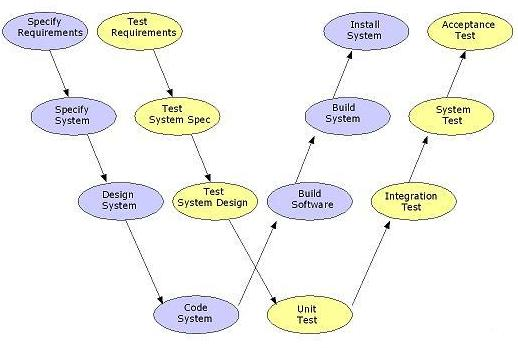
\includegraphics[scale=0.5]{img/Wmodel3.JPG}}
\caption{Model W}
\label{fig:wmodel}
\end{figure}

Praktyczne zastosowanie modelu V powoduje konieczność dostosowania go do aktualnie panujących warunków w organizacji i warunków rynkowych. Jedną z wariacji modelu V jest model W. Model W dostarcza większą władze zespołowi testowemu już w początkowych fazach projektu. Model ten zakłada iż już podczas fazy analizy i projektowania, dostarczane artefakty są wstępnie weryfikowane i walidowane. Model ten zakłada dla faz z lewej części modelu istnienie równoległych faz które je kontrolują, weryfikują i walidują. Tak więc dopiero zaakceptowane artefakty służą jako dane wejściowe do procesu planowania odpowiednich faz związanych z testowaniem.
\paragraph{}
Model ten zakłada iż projekt zostaje testowany jak najwcześniej. Początkowo wykonywane są testy statyczne i prototypowanie pod kątem użyteczności. Testy dynamiczne wykonywane są gdy zaimplementowane są komponent

\paragraph{}
Rozszerzonym wariantem modelu W, jest model "butterfly"\cite{BUTTERFLY}. Model ten zakłada że każdą z faz można podzielić na kilka mikro-iteracji. Każda z iteracji składa się z analizy pod kątem możliwości przetestowania, projektu testów i ich wykonania. 
\begin{figure}[h]
\centerline{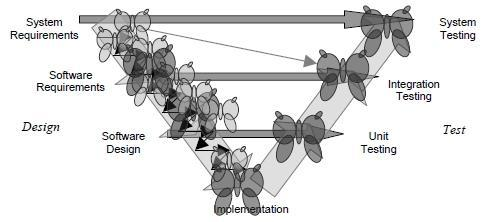
\includegraphics[scale=0.5]{img/butterflymodel2.JPG}}
\caption{Model "butterfly"}
\label{fig:vmodel}
\end{figure}
\subsection{Modele iteracyjne}
Modele iteracyjne w przeciwieństwie do modeli tradycyjnych zakładają podzielenie projektu na mniejsze części które są tworzone niezależnie. Można wydzielić dwa typy modeli iteracyjnych
\begin{itemize}
  \item czysto iteracyjne - co oznacza iż rozwiązane projektowane jest raz, natomiast faza produkcji i testowania dzielona jest na mniejsze części
  \item przyrostowe - co oznacza iż projekt dzielony jest na mniejsze części i każda z części posiada oddzielną fazę projektowania, implementacji i testowania. Każda z części dodaje nowe funkcjonalności
 
\end{itemize}
 Modele iteracyjne poprzez podział na podprojekty wymagają od zespołu testerskiego wykonyania regresji począwszy od drugiej iteracji. Regresja ta ma na celu sprawdzenie czy nowo dodany kod nie wprowadził błędów do wcześniej oddanego i przetestowanego rozwiązania.
\subsubsection{RAD}
Rad czyli Rapid Aplication Development (szybkie tworzenie oprogramowania) to model który zakłada podział projektu na mniejsze
 niezalezne moduły ktore mogą byc implementowane przez rozdzielne zespoly równolegle. Zespoly w trakcie pracy używaja gotowych komponentów i narzedzi do generowania kodu dostosowując je do indywidualnych potrzeb projektu. Model zakłada że rozwiazanie może zostać oddane w bardzo krotkim czasie to jest 30-90 dni roboczych.

Faza testowania zakłada iż gotowe komponenty używane w projekcie są już przetestowane. Testami należy pokryć kustomizacje rozwiązania. 
\paragraph{}
Rozwiązanie to sprawdza się w sytuacji gdy produkt jest mocno ograniczony czasowo, natomiast jakość i wydajność nie są priorytetem. Wadą rozwiązania jest niska wydajność rozwiązania powodowana używaniem generycznych komponentów. Wydajność obniża także niezależnością między zespołami które produkując swoje rozwiązanie nie kalibrują go z rozwiązaniem równoległych zespołów.
\paragraph{}
Zdarza się iż oprogramowanie wyprodukowane poprzez ten model jest używane jako prototyp za pomocą którego projektowane jest końcowe rozwiązanie. Za pomocu modelu RAD tworzone jest więc oprogramowanie aż do pewnego momentu tak by klient mógł skonfrontować swoje przewidywania z działającym oprogramowaniem. Następnie walidowane są wstępne wymagania po czym następuje kontynuacja projektu już z zastosowaniem bardziej formalnych technik.
\subsubsection{Techniki zwinne}
Techiniki zwinne zakładają uproszczenie procesu analizy i projektowania oprogramowania zakładając zmienność wymagań w czasie. Głównymi aspektami zwinnych modeli jest:
\begin{itemize}
  \item zaangażowanie interesariuszy podczas trwania projektu - model ten przewiduje że przynajmniej jeden reprezentant interesariuszy bydzie aktywnym członkiem zespołu. Oznacza to iż zespół projektowy może szybko otrzymać informacje zwrotne na temat projektu
  \item szybka reakcja na zmienianiające się wymagania - w ramach iteracji tworzone są tylko te funkcjonalności które wchodzą w jej skład. Nie są podejmowane kroki mające przygotować system do lżejszej integracji z funkcjonalnościami planowanymi w przyszłości 
  \item uproszczenie dokumentacji i wymagań - nie istnieje sformalizowany proces dokumentacji, część zespołów stosouje jedynie dokumentacje kodu.
  \item idea wspólnego kodu - każdy członek zespołu ma prawo poprawić kod innej osoby
  \item duży nacisk na zapewnienie jakości podczas fazy implementacji - stosowane są techniki mające zapewnić wysoką jakość rozwiązania. Jest to np. TDD czyli pisanie testów komponentowych przed rozpoczęciem implementacji
  \item ciągła integracja i automatyczna regresja - implementacja jest sprężona z automatycznymi narzędziami do budowania produktu. Oznacza to iż autoatycznie po dodaniu nowego kodu do repozytorium produkt jest budowany i może zostać objęty automatyczną regresją bądź manualnymi testami.
\end{itemize}
Projekt zwinny niesie ze sobą również nowe wyzwania dla zespołu testerskiego. Jedym z aspektów jest nowa forma statycznego przeglądu kodu, zespoły zwinne stosują programowanie w parach które zakłada iż podczas pisania kodu, programiści pracują we dwójke zmieniając się, przy czym w danym czasie jedna osoba tworzy kod, natomiast druga kontroluje i szuka lepszych rozwiązań. Forma ta zakłada iż kod taki jest już wstępnie zweryfikowany i nie wymaga innych formalnych metod. 
Bardzo ważnym aspektem jest dobra komunikacja w zespole, pomiędzy programistami i zespołem testerskim. W wyniku braku obszernej dokumentacji, pewne informacje przekazywane są bezpośrednio. Rola testera sprowadza się często do funkcji doradczych i pełni on często aktywną rolę już w fazie implementacji.
Zapewnienie automatycznej regresji jest kluczowe dla projektów zwinnych. Musi ona być wykonana po zakończeniu każdej z iteracji by uzysać pewność czy nie wprowadziła ona błędów do wcześniejszych rozwiązań
\section{Typy strategii}
Typ strategii określa jakie testy będą wykonywane na różnych poziomach testowania. Celem jest stworzenie przypadków użycia i dobór konkretnych skryptów tak by zapewnić oczekiwany poziom jakości przy minimalizacji kosztów i czasu.
\paragraph{}
Pierwszą z opisywanych grup strategii jes grupa strategii analityczne. Zakładają one iż dany wejściowymi są artefakty powstałe podczas tworzenia oprogramowania które następnie poddawane są analizie. Artefaty używane do analizy to na przykład dokumentacja, kod źródłowy, przypadki użycia, lista funkcjonalności.

Najczęściej spotykanami strategiami analitycznymi jest strategia sterowana ryzykiem i strategia sterowana funkcjonalnością. Zostaną one przedstawione poniżej.

Dla testowania sterowanego funkcjonalnością, jako dane wejściowe używane są funkcjonalności. Projektowanie fazy testowania ma na zadanie pokrycie testami wszystkich wymienionych funkcjonalności. Jest to proces który złożony z dwóch części: walidacji wymagań i identyfikacji przypadków użycia na podstawie wymagań. 
\paragraph{}
Wymagania walidowane są pod kątem wieloznaczności, wzajemnego wykluczania się, niepełnego opisu. Nieprecyzyjne opisy są uzupełniane a dwuznaczności eliminowane. Wyeliminowanie wieloznaczności wymaga obecności interesariuszy, programistów i testerów ponieważ każda z tych grup może interpetować funkcjonalności w inny sposób co prowadzi do kosztowych błędów w projekcie.
\paragraph{}
Kolejnym krokiem jest wygenerowanie minimalnej ilości przypadków użycia które pokryją wszystkie funkcjonalności. Na ich podstawie powstają skrypty testowe. Do tego celu tworzony jest diagram przyczyna-efekt. Służy on do zobrazowania na podstawie funkcjonalności wpływu stanu systemu na oczekiwany rezultat. Po lewej stronie diagramu umieszczane są możliwe warunki wejściowe, po prawej oczekiwany efekt. Pomiędzy dwoma warstwami zachodzą relacje które mogą posiadać warunki logiczne takie jak: i, lub, nie. Dodatkowo można wyróżnić warunki wejściowe których odpowiednia wartość powoduje iż wartość pozostałych elementów nie jest brana pod uwagę, wartości te możemy więc zamaskować. Na podstawie diagramu tworzona jest tabela decyzyjna która jest źródłem przypadków użycia.
\paragraph{}
Drugą ze strategii analitycznch jest testowanie sterowane ryzykiem. Zakłada one iż najpierw wykonujemy te testy które dotykają obszarów oprogramowania mających największe ryzyko.  Dobór ryzyka polega na priorytyzacji zdarzeń które mogą wystąpić, mających negatywny wpływ na jakość oprogramowania.
Priorytezacja polega na przypisaniu do każdego ze zdarzeń prawdopodbieństwa jego wystąpienia i wpływu jaki ma na jakość oprogramowania. Wartości te mogą być liczbowe ( np 1-10), bądź dyskretnie ustalone (np. małe, średnie, duże). Następnie dla par ryzyko-wystąpienie przypisywana jest końcowa wartość ryzyka. Ważne jest aby w trakcie trwania projektu na bieżąco monitorować aktualny stan ryzyka, gdyż może on zmieniać się w czasie.

Istnieje kilka wyróżnionych domen do których można przyporządkować poszczególne ryzyka. Spis kategorii pozwala dostrzeć pewne powszechne ryzyka które mogą zostać pominięte
Kategorie ryzyka:
\begin{itemize}
  \item funkcjonalność
  \item wydajność
  \item obciążenie
  \item instalacja i deinstalacja
  \item zarządzanie
  \item regresja
  \item użyteczność
  \item jakość danych
  \item obsługa błędów
  \item obsługa daty i czasu
  \item internacjonalizacja
  \item konfiguracja dla różnych środowisk uruchomieniowych
  \item sieci
  \item bezpieczeństwo
  \item dokumentacja
\end{itemize}

\paragraph{}
Drugim typem strategii są te oparte na modelu oprogramownia.  Istnieją programy wspierające tego typu strategie które generują przypadki użycia bezpośrednio z modelu, tak więc nie muszą być one tworzone manulanie.
Model systemu to między innymi diagramy przejścia, model domeny, maszyna stanów skończonych. Przepływ dla tego typu strategii wygląda następująco: system, model systemu, skrytpy testów, konkretnie wywołania testów.
\paragraph{}
Trzecim typem strategii są strategie metodyczne. Dla tego typu strategii, projekt testów powstaje na podstawie zdefiniowanej metody. Przykładem metody może być metoda uczenia która polega na stworzeniu listy pomocniczej która składa się z pytań na które należy odpowiedzieć podczas projektowania i zagadnień które należy poruszyć. Lista taka powstaje na podstawie przeglądu wcześniejszych błędów, wiedzy dziedzinowej, konsultacji eksperckich. Strategia metodyczna może też to być strategia korzystająca z metod opisanych standardami. Przykładowo standard IBM zakłada podział testowania na kategorie takie jak: użyteczność, funcjonalności, wersje językowe, dostępność, wydajność, obciążenie, dokumentacja, instalacja.
\paragraph{}
Strategie zorientowane procesowo, są to strategie których trzonem jest ogólnie przyjęty standard testowania. Przykładem takich strategi może być IEEE 82, czy standardy dla przemysłu lotniczego. Adaptacja strategi wymaga dostosowania ich do specyfiki produktu. Innym przykładem mogą być opisane strategie testowania zwinnego, które zakładają mocną automatyzację procesu testowania i odporność na zmianę nawet w późnym etapie projektu. Automatyzacja testowania zakłada cykliczne wykonywanie grup testów, dla których dane wejściowe są losowe.
\paragraph{}
Dynamiczne strategie testowe, zakładają zmiejszony nakład na projektowanie i planowanie fazy testowej. Strategia ta zakłada adoptowanie sposobu testowania do aktualnych warunków. Przypadki testowe tworzone są na bieżąco przy czym głównie wykonywane są testy eksploracyjne i testy eksperckie. Testerzy wraz z poznawaniem systemu, ustalają priorytety i scenariusze.
\paragraph{}
Strategia sterowana specyfiką testowania oprogramowania zakłada iż każdy produkt zawiera w sobie błędy. Przyjmowane są z góry nałożone dolne limity błędów które może zawierać oprogramowanie. Testowanie prowadzone jest do czasu aż limity nie zostaną osiągnięte. Oznacza to iż dynamicznie dokładane są nowe testy.
\paragraph{}
Strategie testów regresyjnych, są to strategie ktore mają zapewnić iż nie został wprowadzony błąd w działającej i przetestowanej już funkcjonalności. Największy nacisk kładziony jest w modelu iteracyjnym i dla produków które posiadają wiele wydań. Błędy regresji mogą występować w trzech rodzajach:
\begin{itemize}
  \item błąd bezpośrednio wprowadzony przez poprawę defektu lub wprowadzenie nowej funkjonalności
  \item błąd który objawił się dopiero po naprawie defektu lub dodaniu nowej funkjonalności
  \item  błąd który pojawił się w innym obszarze produktu lub systemu w związku z nową funkcjonalnością lub poprawą defektu,
\end{itemize}

\paragraph{}
Istnieje kilka strategii regresji. Pierwsza strategia to wykonywanie wszyskich testów wywoływanych podczas poprzeniej iteracji bądź wersji systemy. Strategia ta związana jest z dużymi kosztami tak więc najczęściej polega ona na wywoływaniu wszystkich testów automatycznych i automatyzacji tych testów które prawdopodobnie będą powtarzane w przyszłości. Drugą opcją jest wykonanie wybranej puli testów. Dobór testów dokonywany jest na różne sposoby, może to być przydział ekspercki polegający na analizie tego co mogło się zmienić. Może to być także testowanie które zakłada większą aktywność dla elementów obarczonych większym ryzykiem bądź tych które mają krytyczne znaczenie biznesowe lub znaczenie dla bezpieczeństwa. Powinny zostać również wykonane te testy które absorbują cały system, tak by potwierdzić że wszystkie elementy wpsółpracują poprawnie.

\section{Typy testów}
Testy oprogramowania można dzielić według różnych kategorii. W niniejszej pracy przedstawiony zostanie podział ze względu na poziom i typ testów.
 
\subsection{Podział ze względu na obszar zastosowania}
\subsubsection{Testy komponentowe}
Testy komponentowe są to testy które szukają defektów i weryfikują funkcjonalności na poziomie pojedyńczych klas, modułów kodu źródłowego. które mogą być uruchamiane i testowane niezależnie. Testy komponentowe wykonywane są często w izolacji z innymi częściami systemu. Klasy dostarczające dane, silniki bazodanowe, zastępowane są przez specjalne obiekty które naśladują ich działanie. Technika ta ma na celu zapewnienie iż wykrycie błędu podczas testowania określonego modułu nie jest spowodowane błędem wynikającym z błednych danych pochodzących z modułów zależnych które nie są aktualnie obiektem testu. Testy takie charakteryzują się wysokim zwrotem inwestycji. Dodatkowo stanowią dokumentacje jako przykład użycia kodu źródłowego.

Testy komponentowe najczęściej wykonywane są podczas fazy implementacji. Wykonywane i tworzone są przez zespół programistyczny, co więcej najczęściej osoba która tworzy komponent piszę również do niego test. Dobrą praktyką jest by osoba inna niż autor zweryfikowała czy stworzone testy pokrywają zaimplementowaną funkcjonalność, zdarza się też iż test pisane są przed implementacją. Błędy znalezione podczas testów komponentowych najczęściej nie są logowane ponieważ występują przed formalnym oddaniem kodu źródłowego i zatwierdzeniem go.

\subsubsection{Testy integracyjne} 
Pojedyncze moduly ktory przeszly przez faze testow jednostkowych sa laczone z wieksze grupy dla ktorych wykonywane sa testy zgodnie z planem testow

Celem testow integracyjnych jes weryfikacja spelnienia funkcjonalnosci, niezawodnosci, wydajnosci na poziomie wiekszym niz pojednynczy komponent. Testowane sa wieszke grupy logiczne ktore dostarczaja konkretna funkcjonalnosc. Główną metodą testowania są testy czarno-skrzynkowo, co więcej osoby wykonujące testy najczęściej nie posiadają informacji o sposobie działania kodu.

Istniejie kilka typow testow integracyjnych ktore można wyróżnić ze względu na poziom izolacji modułów.

Pierwszym typem są testy zależne od całości systemu. Przed przystąpieniem do testowania zakłada się iż całość systemu jest dostarczona i może zostać zintegrowana.  Podczas testowania, używane są prawdziwe implementacje wszystkich potrzebnych modułów. Testowanie tego typu daje pewność iż system działa poprawnie używając prawdziwych komponentów. Głównymi wadami jest to iż testy takie można rozpocząć tylko wtedy gdy gotowy jest cały system, co może nastąpić bardzo późno w procesie tworzenia oprogramowania. Problemem jest także izolacja defektu.

Drugim typem testów, przeciwnym testowaniu całościowemu jest testowania polegające na podzieleniu fazy testów integracyjnych na mniejsze fazy z których każda zakłada testowanie każdej pary modułów. Testowanie tego typu zakłada iż tylko testowana para musi być realnym oprogramowanie, reszta systemu jest symulowana. Testowanie tego typu wymaga dostarczenia symulatorów i wspierania ich podczas kolejnych wydań systemu. Zaletą tego typu testu jest możliwość rozpoczęcia testów już gdy zespół programistyczny dostarczy gotowy kod dwóch modułów które z sobą współpracują. Wydzielenie tylko dwóch modułów pozwala także na wysoką izolacje defektów. Wadą jest wysoki kosz i czas trwania tego typu testów gdyż pewne testy powtarzane są dla różnych par modułów.

Pomiędzy dwoma wcześniej opisanynymi podejściami istnieje podejście hybrydowe. Polega ono na łączeniu modułów w grupy niższego poziomu które są wzajemnie testowane. Następnie grupy niższego poziomu łączone są w grupy wyższego poziomu które są wzajemnie testowane. Końcowym etapem może być test integracji całego systemu.
\subsubsection{Testy systemowe}
System jest to zbior zintegrowanych komponentow ktore wspolnie dostarczaja okreslonych wymagan. W skład systemu wchodzi także całe środowisko uruchomieniowe, sprzęt, oprogramowanie zewtnętrzne. Testowanie systemowe jest okreslane jako faza testow ktore sprawdzaja kompletny w pelni zintegrowany system ktory działa na środowisku końcowym lub zbliżonym do końcowegp. Testy te sprawdzaja zgodnosc z okreslonymi wymaganiami takimi jak: funkcjonalnosc, niezawodnosc itp
Faza ta powinna zostac wykonana po testach komponentowych i integracyjnych i może sprawdzać wymagania zarówno funkcjonalne i niefunkcjonalne.
Testy systemowe najczęściej wykonywane są manualnie na podstawie zdefiniowanego planu, przy czymś część testów takich jak testy wydajnościowe mogą być wspomagane automatycznie.
Testy systemowe zakładają iż większość negatywnych scenariuszy takich jak podanie błędnych zdanych sprawdzone zostało podczas faz wcześniejszych testów tak więc testowanie systemowe skupione jest na weryfikacji pozytywnych scenariuszy. 
Testy systemowe powinny być przeprowadzone przez niezależny zespół który raportuje do kierownika niezależnego od departamentu produkcji. 

\subsubsection{Testy akceptacyjne}
Testy akceptacyjne to są takie testy o których będę musiał napisać

\subsection{Podział ze względu na typ}
\subsubsection{Testy funkcjonalne}
\subsubsection{Testy niefunkcjonalne}
\chapter{Określenie problemu} % (fold)
\label{cha:okreslenie_problemu}

W rozdziale zdefiniowany zostanie problem badawczy oraz dokonany zostanie szczegółowy przegląd  podobnych problemów i ich rozwiązań. Ostatecznie postanowiona zostanie teza niniejszej pracy.

\section{Definicja problemu} % (fold)
\label{sec:definicja_problemu}

Tematem pracy jest stworzenie aplikacji wspierającej proces zapewnienia jakości produktu informatycznego. Istnieje wiele różnych aplikacji które wpisują się w tematykę testowania oprogramowania i wspierają ten proces w różnych fazach i aspektach. Założeniem pracy jest stworzenie aplikacji służącej do przechowywania, wersjonowania i wykonywania ręcznych testów.

Odwołując się do wcześniejszych informacji, aplikacja przeznaczona jest do każdego z typów wytwarzania oprogramowania. Typem testów które znajdować się mają docelowo w aplikacji są testy integracyjne i testy systemowe. Charakterystyka testów może być zarówno funkcjonalna jak i niefunkcjonalna, należy jednak mieć świadomość i testy niefunkcjonalne przez swą złożoność mogą nie być możliwe do wykonania manualnego.

Specyfiką aplikacji której projekt i implementacja przedstawione będą w niniejszej pracy jest zapewnienie użyteczności do systemów które posiadają wiele wydań a proces wytwarzania oprogramowania zbliżony jest do modelu inkrementacyjnego. Systemy takie wymagają przeprowadzenia strategii testowej dla każdej inkrementacji oprogramowania. Globalnie dla całego wydania istotne jest to by zbiór testów brany z wszystkich wykonanych strategii pokrywał nową funkcjonalność i zapewniał regresję poprzednich wydań. Dodatkowo autor zakłada iż aplikacja wspiera systemy które dedykowane są na wiele urządzeń. Powoduje to zwiększenie ilości możliwych przypadków testowych dla wydania systemu. 

\begin{equation}
TC_{mix} = TC * D
\end{equation}
	\begin{itemize}
		\item $TC_{mix}$ -- ilość kombinacji przypadków testowych
		\item $TC$ -- ilość przypadków testowych
		\item $D$ -- ilość urządzeń
	\end{itemize}




Powołując się na wiedzę z zagadnień testowania oprogramowania, można stwierdzić iż niemożliwe jest testowanie wszystkich kombinacji przypadków użycia i urządzeń. Celem zapewnienia najwyższej jakości produktu a zarazem zminimalizowania kosztów testów stosowana jest strategia sterowana ryzykiem. Dla przypomnienia polega ona na określeniu które funkcjonalności objęte są najwyższym ryzykiem w aktualnym wydaniu produktu. Powoduje to iż testy odnoszące się do najbardziej ryzykownych funkcjonalności otrzymują najwyższy priorytet. Analogicznie ryzyko nalaży zastosować dla urządzeń dla których produkt jest dedykowany.

W książce pisało o tym że programy powinny móc się integrować, myślę że jest to ważne i można trochę o tym napisać żeby było miło i sympatycznie
\section{Podobne problemy i ich rozwiązania}
Tutaj opiszę typy programów wspierających proces testowania według ISTB.

Następnie wrzucę screenshoty z dwóch konkurencyjnych programów
\chapter{Programy wspierające prosces testowania}
Istnieje wiele programów wspierających proces testowania, przydatkych w różnych fazach tego procesu.
\chapter{Analiza problemu}














